\documentclass[11pt]{article}
\usepackage[margin=2.4cm]{geometry}
\usepackage{graphicx,booktabs,float,xcolor,amssymb}
\usepackage[hidelinks]{hyperref}
\usepackage{helvet}\renewcommand{\familydefault}{\sfdefault}
\usepackage{tcolorbox}
\newcommand{\Mw}{M\textsubscript{w}}
\title{\textbf{Two large intraslab earthquakes of the Calama--San Pedro de Atacama
cluster:\\the 2026 \Mw~6.9 and 2024 \Mw~7.4 events\\
\large moment tensors, finite-fault models, and the nodal-plane question at 109--127 km depth}}
\author{M.-S. Seo\\ \small analysis pipeline: MTUQ (point-source moment tensor) + WISP (kinematic finite fault)}
\date{12 July 2026}
\begin{document}\maketitle

\begin{abstract}
We determine point-source moment tensors (MT) and kinematic finite-fault models (FFM) for the
two most recent large earthquakes of the Calama--San Pedro de Atacama intermediate-depth
cluster in northern Chile: the 2026-05-25 \Mw~6.9 Calama event (109~km deep; Part~I) and the
2024-07-19 \Mw~7.4 San Pedro de Atacama event (127~km deep; Part~II), using identical
teleseismic-only protocols. The pair turns out to be a controlled experiment in what
teleseismic data can and cannot resolve at these depths: for the compact 2026 rupture the two
nodal planes are indistinguishable (misfits within 1.6\%), whereas for the $\sim$4$\times$
larger 2024 rupture the body waves alone discriminate decisively --- the steep plane fits
$\sim$10\% better, independently confirming the near-field-based verdict of Jia et~al.\ (2025)
against the plane adopted by the USGS operational finite-fault model.

Part~I in detail: for the 2026 event ---
an intraslab normal-faulting rupture inside the subducted Nazca plate for which USGS
published moment tensors but no finite-fault model. Using 26 teleseismic GSN stations, our
final moment tensor (\Mw~6.90, strike/dip/rake $=$ 194/16/$-$83, with conjugate plane
7/74/$-$92) lies 8.4$^\circ$ (Kagan angle) from the USGS W-phase solution and fits both the
25--60~s body waves (variance reduction 71.9\%) and the 50--100~s surface waves (67.2\%)
better than the USGS mechanism itself evaluated on the same data. The finite-fault model
resolves a single compact asperity --- on the preferred (shallow) plane a thin slip lens
with 0.70~m peak confined to 105--113~km depth, a single
$\sim$15-s moment-rate pulse, subshear rupture --- with the conjugate planes indistinguishable
in misfit, as expected for a compact deep rupture viewed teleseismically. Depth-phase-sensitive
estimates (finite-fault slip centroid 106.5~km; long-period body-wave depth scan 117~km; USGS
body-wave MT 111~km; hypocentre 109~km) place the best-constrained centroid depth at
$\sim$105--115~km. Beyond the source parameters, this event provided a controlled experiment
in \emph{how standard teleseismic source inversion fails at intermediate depth} --- through
depth-phase interference in short-period body-wave windows and through a silent truncation of
finite-fault surface-wave Green's functions --- and how each failure is diagnosed and fixed. A
first-motion polarity anomaly at five near-nodal stations independently discriminates between
our mechanism and the USGS solution, favouring ours.
\end{abstract}

\begin{tcolorbox}[colback=gray!8,colframe=gray!60,title=\textbf{Plain-language summary}]
A magnitude-6.9 earthquake occurred 109~km below the city of Calama, inside the oceanic
(Nazca) tectonic plate that is sinking beneath South America. Earthquakes this deep happen
\emph{inside} the sinking plate, not on the boundary between plates, and are pulled apart by
the weight of the plate's deeper portion --- our analysis confirms this ``slab-pull'' stretching
almost exactly along the direction the plate is sinking. Using seismometers thousands of
kilometres away, we recovered how the fault is oriented, how much it slipped (up to
$\sim$0.9~m over a patch a few tens of km across, in about 15 seconds), and how deep the
rupture was. Two technical traps specific to deep earthquakes --- both of which initially
produced confident but wrong answers --- are documented step by step, with the checks that
caught them, so that the workflow can be reused by non-specialists on future events.
\end{tcolorbox}

\part*{Part I --- The 2026-05-25 Calama \Mw~6.9 (us6000t04s)}
\section{Tectonic setting}
Beneath northern Chile the oceanic Nazca plate converges with South America at roughly
7~cm/yr and subducts along the Chile trench, dipping eastward beneath the Atacama forearc
and the active volcanic arc (Figure~\ref{fig:map}). Seismicity here occurs in three distinct
habitats: shallow megathrust earthquakes on the plate interface (e.g., the 1995 \Mw~8.0
Antofagasta and 2014 \Mw~8.2 Iquique events), crustal earthquakes in the overriding plate, and
\emph{intermediate-depth intraslab} earthquakes (70--300~km) inside the subducted plate itself.
The 2026 Calama event, at 109~km depth directly below the arc-front longitude, belongs to the
third class --- the same family as the 2005 \Mw~7.8 Tarapac\'a earthquake ($\sim$95~km deep,
normal faulting, $\sim$500~km to the north), which demonstrated that this part of the slab can
host large, damaging ruptures far from the plate boundary.

\textbf{A century of large intraslab earthquakes around this event}
(Figure~\ref{fig:regional}): the USGS catalog holds 80 M$\geq$6 events since 1900 at
60--300~km depth in this region, and the 2026 earthquake is the newest member of a
\emph{persistent cluster of large events at 100--130~km depth between Calama and San Pedro
de Atacama} (we deliberately avoid the term ``nest'', which in the strict sense --- Bucaramanga,
Vrancea, Hindu Kush --- denotes an \emph{isolated} compact volume of exceptionally high
sustained activity; this concentration lies \emph{within} the continuous, highly active
Wadati--Benioff band rather than isolated from it) that has
produced M6.8 events in 1916, 1962, 2005 and 2020, the \textbf{2024 M7.4 San Pedro de
Atacama earthquake} (normal faulting at 127~km, only $\sim$80~km ESE of the 2026 epicentre),
and above all the \textbf{1950 ``Calama'' earthquake (M8.2 at 114~km)} --- the largest
intermediate-depth event ever recorded in Chile, interpreted as down-dip tensional rupture of
a \emph{near-vertical} plane cutting much of the slab's thickness (strike/dip/rake
$\approx$350/88/$-$90, two subevents, stress drop $\sim$10~MPa) --- though that plane
inference rests on long-period body-wave modelling of 1950-era analog records alone; with no
local aftershock network or geodesy, it is suggestive rather than firmly constrained. Farther north, the 2005 Tarapac\'a M7.8
ruptured a \emph{sub-horizontal} plane (50$\times$40~km$^2$, slip locally 13~m, average
stress drop $\sim$15~MPa, rupture velocity $\sim$4.5~km/s). A second, deeper cluster
(200--250~km, beneath the Chile--Argentina--Bolivia border) produced the 1957 M7.7, 1993 M7.0,
2000 M7.2 and 2022 M6.8 events. High-resolution local catalogs (IPOC; $>$100{,}000 relocated
events) show why the 100--130-km band is special: the double seismic zone of the shallower
slab merges near 80--100~km into a single 25--30-km-thick seismogenic volume in which
seismicity rate and moment release sharply increase --- our event, its slip lens only
$\sim$8~km thick, ruptured comfortably inside that volume.
\begin{figure}[H]\centering
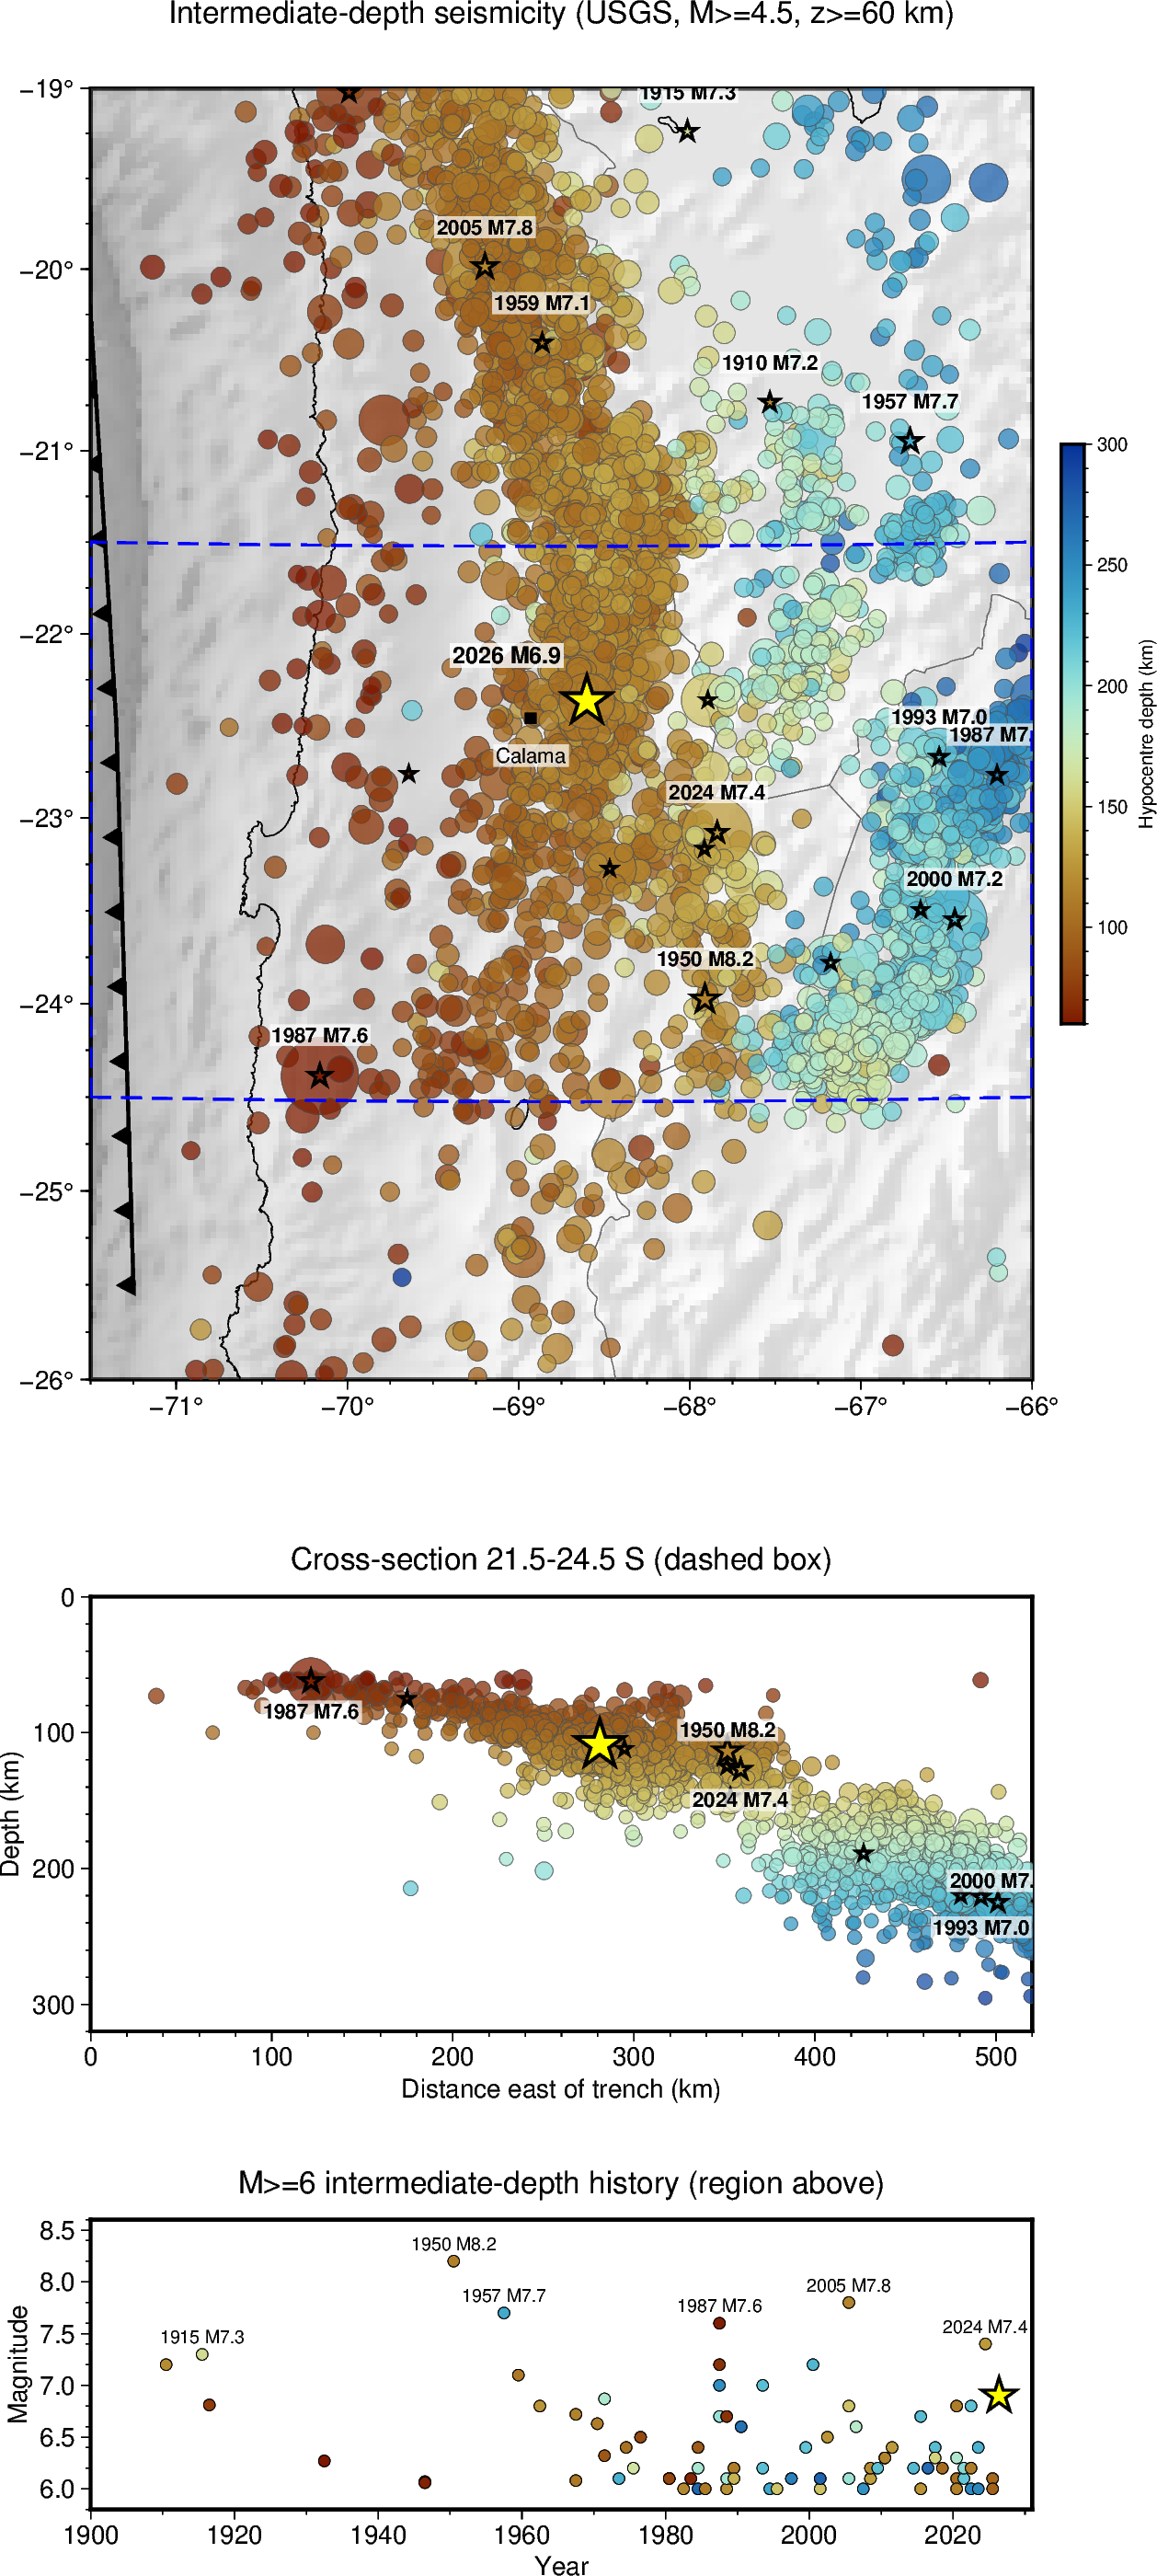
\includegraphics[width=.88\textwidth]{fig_regional_seismicity.png}
\caption{Regional intermediate-depth seismicity. Top: USGS M$\geq$4.5 events (z$\geq$60~km,
1960--2026) coloured by depth; stars: M$\geq$6.8 since 1900 (labelled if M$\geq$7); yellow
star: the 2026 event. Middle: trench-perpendicular cross-section of the dashed band, showing
the Wadati--Benioff zone and the 100--130-km cluster hosting the 1950 M8.2, 2024 M7.4 and 2026
events. Bottom: magnitude--time history of M$\geq$6 intermediate-depth events.}
\label{fig:regional}
\end{figure}

Intermediate-depth earthquakes cannot be explained by ordinary frictional sliding --- at these
pressures rock should deform by flow, not stick-slip --- and are generally attributed to
\emph{dehydration embrittlement}: water released by minerals in the sinking oceanic crust and
mantle raises pore pressure and re-enables brittle failure, often re-activating the normal
faults created at the outer rise before subduction. Mechanically, the deeper slab hangs off
the shallower slab, stretching it down-dip (``slab pull''). Our solution matches this picture
quantitatively: the tension (T) axis of the final mechanism plunges 29$^\circ$ toward
N98$^\circ$E --- within a few degrees of the local slab down-dip direction --- i.e., the slab
snapped in down-dip extension. Both nodal planes (a steep east-dipping plane, 7/74, and a
gently west-dipping plane, 194/16) are geometrically plausible reactivated structures; as
shown in \S\ref{sec:ffi}, teleseismic data cannot choose between them for a rupture this
compact, and we discuss both.

\begin{figure}[H]\centering
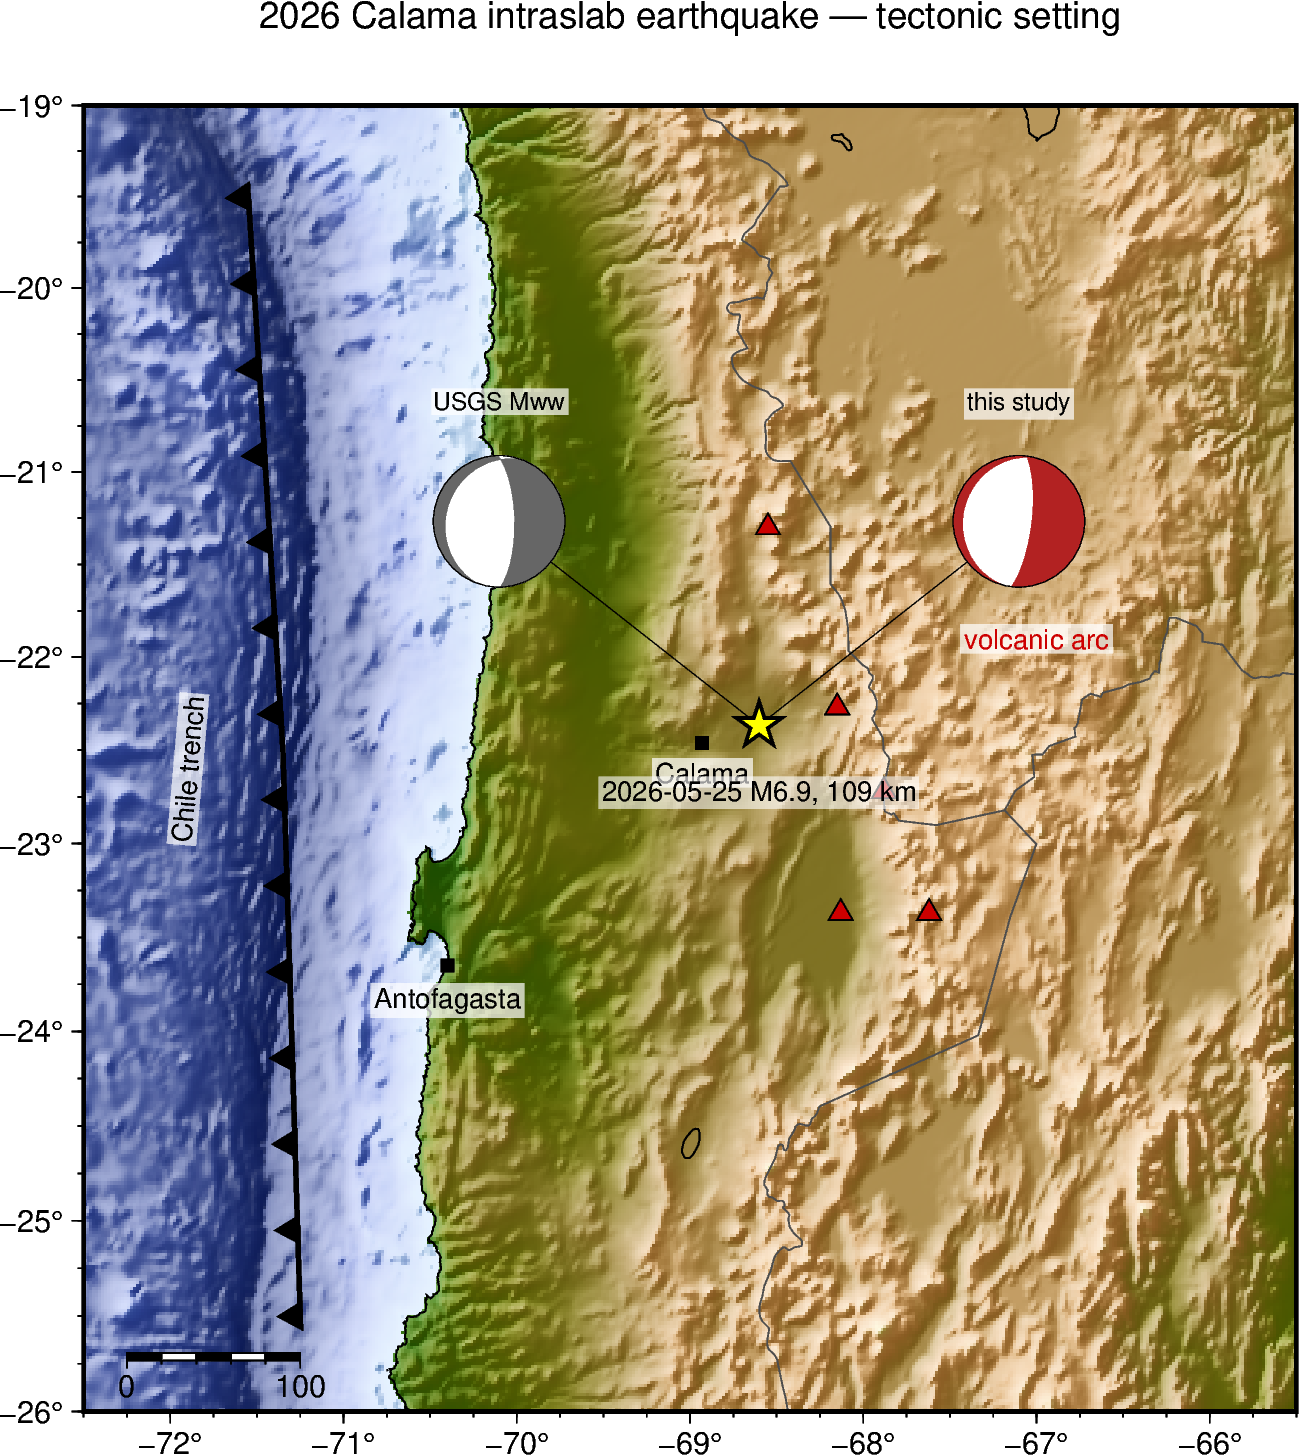
\includegraphics[width=.9\textwidth]{fig_tectonic_map.png}
\caption{Tectonic setting. The Nazca plate subducts eastward at the Chile trench (toothed
line); red triangles mark main-arc volcanoes. The star is the 2026 Calama epicentre
(hypocentre 109~km); focal spheres compare the USGS W-phase mechanism (grey) with this
study's (red) --- both normal-faulting, 8.4$^\circ$ apart.}
\label{fig:map}
\end{figure}

\section{Methods in brief (a primer)}
\label{sec:primer}
Readers familiar with source inversion can skip to \S\ref{sec:data}.

\textbf{Moment tensor (MT).} A point-source description of an earthquake: the fault
orientation (strike/dip/rake), the size (moment $M_0$, expressed as \Mw), and the source type.
It is estimated by generating synthetic seismograms for trial mechanisms (using Green's
functions --- the Earth's response to an impulsive source in a reference velocity model, here
ak135) and grid-searching for the mechanism whose synthetics best match the observations. A
\emph{double couple} (DC) is the special case of pure slip on a planar fault; every DC has
two mathematically indistinguishable \emph{conjugate} fault planes, so distinguishing the real
plane always needs extra information beyond the radiation pattern. Our searches use MTUQ,
which implements the cut-and-paste (CAP) strategy: body-wave and surface-wave portions of each
record are windowed, filtered into separate period bands, and allowed small independent time
shifts, so that imperfect knowledge of Earth structure does not corrupt the mechanism estimate.

\textbf{Finite-fault model (FFM).} Relaxes the point-source approximation: the fault plane is
divided into subfaults, each with its own slip, rake, rupture-arrival time and rise time,
inverted from waveforms (here with WISP, the USGS operational code, using teleseismic P, SH,
Rayleigh and Love waves). The output is a slip map and a moment-rate function (how fast moment
was released versus time).

\textbf{Depth phases --- the key concept at 109 km.} Besides the direct P wave, a deep source
sends energy \emph{up}, which reflects off the Earth's surface and follows P down to the same
station: the phase pP (and sP for an up-going S leg). The lag pP$-$P grows with source depth
($\approx$25~s at 109~km) and is the single most depth-sensitive observable in teleseismic
data. Crucially, pP reflects with flipped polarity. Whether a method treats these arrivals as
signal or lets them contaminate its windows decides whether depth helps or hurts --- the
central methodological theme of this study.

\textbf{Fit and comparison metrics.} \emph{Variance reduction} (VR) is the percentage of
waveform energy explained by the synthetics (100\% = perfect; negative = worse than predicting
zero motion). The \emph{Kagan angle} is the single 3-D rotation between two mechanisms
(0$^\circ$ = identical; routine agency solutions for the same event typically differ by
10--20$^\circ$). WISP reports a normalized waveform \emph{misfit} (lower is better); misfits
are comparable \emph{only} between runs inverting the same data with the same wave types.

\section{Data and processing}
\label{sec:data}
\textbf{MTUQ:} 26 three-component GSN broadband stations at 25--75$^\circ$ epicentral distance,
azimuthally distributed. Instrument response was removed to ground displacement with no
water-level stabilization (a water level biases long-period amplitudes --- a lesson from the
companion Venezuela study), data at 2~Hz. \textbf{WISP:} 180 teleseismic channels fetched with
an obspy-based fallback downloader (\texttt{wisp\_fetch\_fallback.py}; the packaged IRIS
discovery endpoint is no longer served), pole-zero response files renamed and headers fixed
with true BH1/BH2 azimuths. Deep-event P is impulsive: $\sim$45--49 P channels pass WISP's
signal-to-noise gate --- in sharp contrast to a same-magnitude shallow event (our Sanriku
study), where \emph{all} P channels failed it. Three surface-wave channels that no model
variant could fit (EDA Rayleigh and Love, PTCN Love --- isolated island paths) were
zero-weighted in the final inversion and are shown grey in the fit figures. Figure~\ref{fig:stations}
shows both station sets. All inversion parameters are listed in Appendix~A.
\begin{figure}[H]\centering
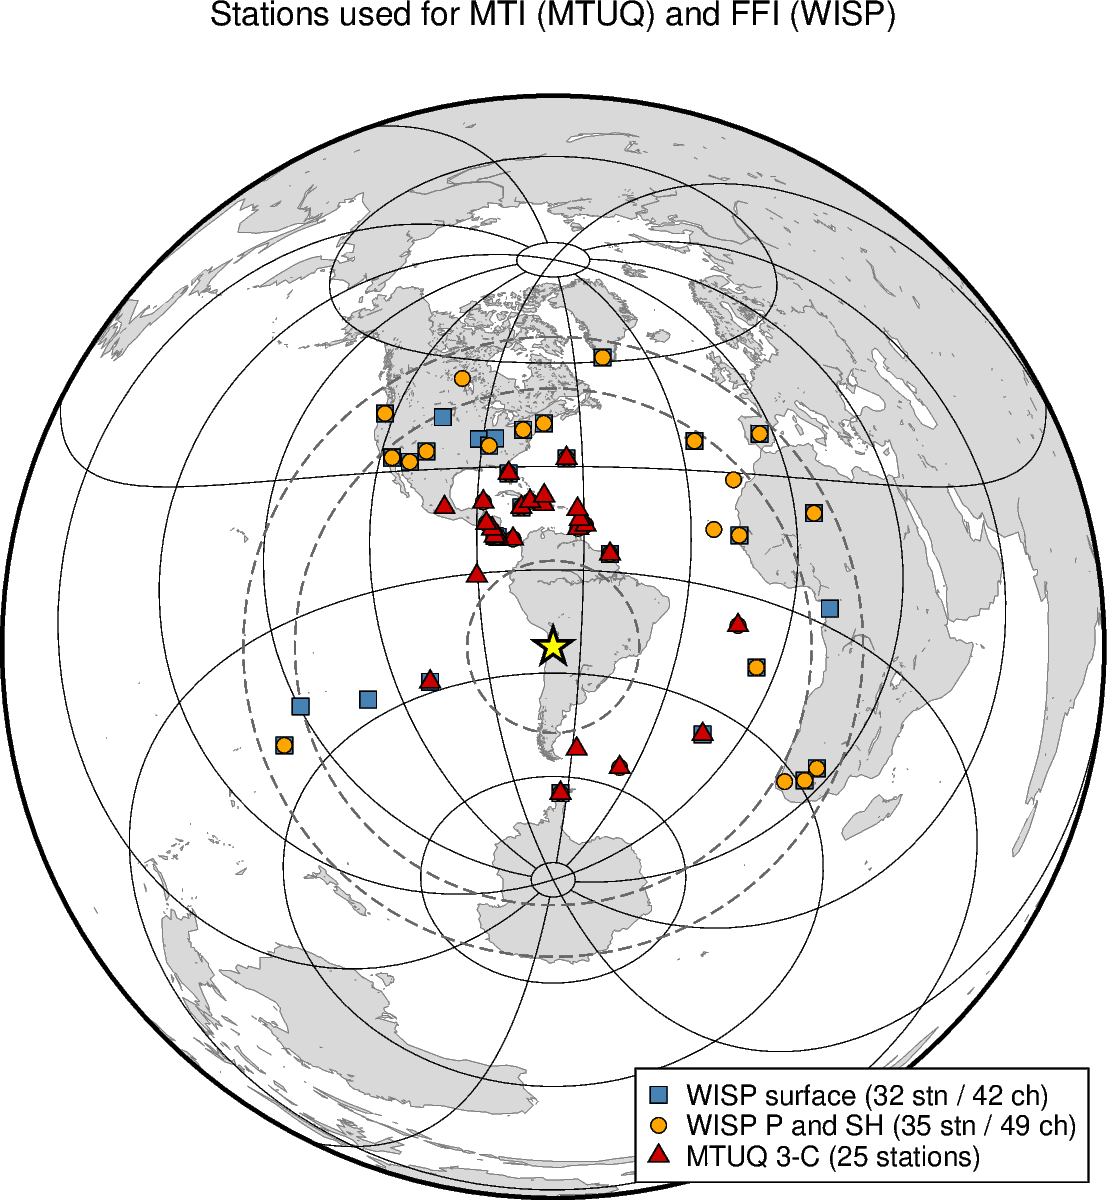
\includegraphics[width=.8\textwidth]{fig_stations.png}
\caption{Stations used. Red triangles: the 25 GSN three-component stations of the MTUQ
inversions (dashed circles: the 25--75$^\circ$ selection window). Orange circles / blue
squares: WISP body-wave (35 stations, 49 P+SH channels) and surface-wave (32 stations, 42
channels; 39 active in the final model) sets. Azimuthal-equidistant projection centred on the
epicentre (star).}
\label{fig:stations}
\end{figure}

\section{Moment tensor: failure, diagnosis, cure}
\label{sec:mt}
Table~\ref{tab:mt} traces the full sequence --- we report it in order because the failure modes
are as reusable as the final numbers.

\begin{table}[H]\centering\footnotesize\setlength{\tabcolsep}{3.5pt}
\begin{tabular}{llllll}\toprule
run & band & \Mw & strike/dip/rake & Kagan vs Mww & note\\\midrule
full MT @109 km & body 10--33 s + SW & 6.80 & 54/18/$-$45 ($w{=}0.905$) & --- & strongly non-DC: red flag\\
DC @109 km & body 10--33 s + SW & 6.75 & 4/75/$+$83 & 85.5$^\circ$ & \emph{reverse} --- the body flip\\
DC + depth (85--125 km) & body 10--33 s + SW & 6.75 & 7/75/$+$79 @85 km & 85.3$^\circ$ & same flip; edge of range\\
DC + depth (55--115 km) & SW only & 6.90 & 208/19/$-$64 @115 km & 3.3$^\circ$ & monotonic: no depth resolution\\
DC @85 km & SW only & 6.90 & 14/75/$-$83 & 17.7$^\circ$ & $\approx$ USGS Mww\\
DC @107 km & body 25--60 s only & 6.90 & 7/82/$-$72 & 26.7$^\circ$ & body waves recovered\\
DC + depth (85--125 km) & body 25--60 s only & 6.90 & 7/80/$-$86 @\textbf{117 km} & 14.9$^\circ$ & \emph{interior} depth minimum\\
DC + depth (85--125 km) & body 25--60 s + SW & 6.90 & 209/20/$-$65 @125 km & $\sim$3$^\circ$ & edge; SW dilutes depth signal\\
\textbf{DC @107 km (final)} & \textbf{body 25--60 s + SW} & \textbf{6.90} & \textbf{194/16/$-$83} &
\textbf{8.4$^\circ$} & all data; 107 km adopted (= WISP centroid)\\
USGS Mww & W-phase & 6.9 & 359/71/$-$97 @85.5 km & 0 & reference\\\bottomrule
\end{tabular}
\caption{Moment-tensor runs, in chronological order. SW = surface waves (50--100~s). Kagan
angles computed with the canonical \texttt{pyrocko} implementation. $w$ is MTUQ's non-DC lune
coordinate.}
\label{tab:mt}
\end{table}

\subsection{The failure}
With the standard teleseismic settings (body waves at 10--33~s in a 40-s window starting at
the P arrival), the DC search converged --- reproducibly, with a clean-looking misfit surface
--- on a \emph{reverse}-faulting mechanism $\sim$85$^\circ$ from every published solution. Data
hypotheses (time-shift clamping; a non-band-limited resampler) were tested and excluded: freshly
re-prepared, Lanczos-resampled data still flipped. The decisive measurement was evaluating the
\emph{USGS} mechanism on our own body windows: VR $= -24\%$. When the accepted answer fits
worse than a flat line, the protocol --- not the Earth, not the data --- is broken. (The
unconstrained full-MT search absorbed the same inconsistency into a nearly pure non-double-couple
source, $w=0.905$: at depth, a strongly non-DC result should be read as a symptom, not a
discovery.)

\subsection{The diagnosis and the cure}
At 109~km the 40-s body window contains P, pP and sP together, and the depth phases carry
3--5$\times$ the direct-P energy with flipped polarity (visible directly in
Figure~\ref{fig:pfits}). Their spacing inside the window is set by source depth, not by the
window's single allowed time shift; and because the rupture spans $\sim$33~km of depth, the
observed ``pP'' is really a $\sim$10-s smear that no single point depth reproduces. A point
source with a simple wavelet is valid only at periods long compared to both the $\sim$15-s
source duration and that smear ($T\gtrsim45$~s), while resolving pP as a distinct pulse
requires $T\lesssim25$~s: \emph{for an \Mw~6.9 at 109~km there is no band where a short-period
point-source treatment both fits the body waves and resolves depth.} The practical cure is to
move the body band to 25--60~s in a 120-s window that holds the whole P+pP+sP group as one
unit ($\pm$10~s shifts, Green's functions at the 107-km centroid). This single change flips
body-wave VR from $-$80.5\% to $+$71.9\% (our mechanism) and $-$24.0\% to $+$67.7\% (USGS),
demotes the spurious reverse mechanism to 18.5\%, and lets a body-only search recover the
correct normal-faulting family. Unexpectedly, the long-period body waves also retain
\emph{interference-shape} depth sensitivity (the composite P+pP+sP waveform changes shape with
depth even though pP is not separately resolved, as in W-phase methods): a body-only depth
scan exhibits a genuine interior misfit minimum at 117~km (Figure~\ref{fig:depth}, right).

\subsection{The final solution}
The joint search (25--60~s body + 50--100~s surface waves, 107~km) yields \textbf{\Mw~6.90,
194/16/$-$83} (conjugate 7/74/$-$92), 8.4$^\circ$ from the USGS Mww --- well within routine
inter-agency scatter --- with VR of 71.9\% (body) and 67.2\% (surface waves), each higher than
the USGS mechanism evaluated on identical data and Green's functions (67.7\%/66.7\%). The
first-motion evidence of \S\ref{sec:polarity} independently favours this small rotation away
from the USGS solution.

\begin{figure}[H]\centering
\includegraphics[width=.46\textwidth]{../../results/mtuq_dcz_calama_swonly/calama_swonly_misfit_depth.png}
\includegraphics[width=.46\textwidth]{../../results/mtuq_dcz_calama_lpbody/calama_lpbody_misfit_depth.png}
\caption{DC misfit vs depth. Left: surface waves only (55--115~km) --- monotonic; 50--100~s
surface waves carry no centroid-depth resolution for a source this deep. Right: body waves
only, 25--60~s band (85--125~km) --- a genuine interior minimum at 117~km.}
\label{fig:depth}
\end{figure}
\begin{figure}[H]\centering
\includegraphics[width=.44\textwidth]{../../results/mtuq_dc_calama_lpbody/calama_lpbody_beachball.png}
\caption{Final DC (194/16/$-$83; body 25--60~s + surface waves, 107~km) and the 26 stations.}
\end{figure}
\begin{figure}[H]\centering
\includegraphics[width=.72\textwidth]{../../results/mtuq_dc_calama_lpbody/calama_lpbody_misfit_dc.png}
\caption{DC misfit surfaces (strike--dip--rake) for the final joint search.}
\end{figure}
\begin{figure}[H]\centering
\includegraphics[width=.85\textwidth,height=.88\textheight,keepaspectratio]{../../results/mtuq_dc_calama_lpbody/calama_lpbody_waveforms.png}
\caption{Waveform fits at the final DC (black = observed, red = synthetic): 25--60~s body
windows (left columns) and 50--100~s surface-wave windows.}
\end{figure}

\section{Finite-fault model}
\label{sec:ffi}
WISP was run in its strict CLI pipeline (automatic model construction, both nodal planes,
teleseismic body + surface waves). Two findings shaped the analysis.

\textbf{A silent Green's-function truncation manufactured a fake plane discrimination.} The
steep plane's automatically built fault (15 down-dip rows) reached 133.6~km --- below the
$\sim$126-km floor of WISP's surface-wave Green's-function bank --- and WISP dropped \emph{all}
surface waves for that plane only, noting it in a single log line. The resulting misfits
(0.114 for the steep plane vs 0.166 for the shallow plane) compared a body-only number against
a body+surface number and made the steep plane appear strongly preferred. After trimming the
fault to 12 rows and refining \textbf{both} planes identically (all quality control and
cross-correlation alignment applied equally, all wave types inverted), the planes are
indistinguishable:

\begin{table}[H]\centering\footnotesize\setlength{\tabcolsep}{4pt}
\begin{tabular}{llllll}\toprule
input mechanism & plane & misfit & peak slip & slip depth extent & slip centroid\\\midrule
USGS Mww & shallow (201/20) & 0.1470 & 0.75 m & 104--115 km & 108.8 km\\
USGS Mww & steep (359/71) & 0.1473 & 0.78 m & 88--121 km & 106.2 km\\
\textbf{this study} & \textbf{shallow (194/16)} & \textbf{0.1461 (0.1402$^\dagger$)} & \textbf{0.70 m} & \textbf{105--113 km} & \textbf{109.3 km}\\
this study & steep (7/74) & 0.1481 (0.1424$^\dagger$) & 0.89 m & 94--121 km & 106.8 km\\\bottomrule
\end{tabular}
\caption{The fair model comparison: two input mechanisms $\times$ two nodal planes, all with
identical fault trimming, quality control, channel set (49 P + 42 surface) and alignment; all
\Mw~6.93. Misfit differences are at the $10^{-3}$ level --- individually not decisive --- but
the best-fitting model is the shallow plane with this study's mechanism, concordant with the
regional precedent (\S\ref{sec:ffi}). $^\dagger$Final values after zero-weighting the three
unfittable island-path surface channels (EDA, PTCN): shallow 0.1402, steep 0.1424 --- the
shallow plane remains marginally preferred under every treatment.}
\label{tab:planes}
\end{table}

Both planes carry the same double couple ($\leq$2$^\circ$ from the USGS Mww). Which is the
real fault? The waveforms cannot say, but three physical arguments can be weighed. (i) The
closest regional analog, the 2005 Tarapac\'a \Mw~7.8 (same slab, $\sim$95~km), was shown by
aftershock geometry and rupture extent to have ruptured its \emph{near-horizontal} plane ---
the NP1-type geometry. (ii) NP1's slip forms a thin subhorizontal lens (104--115~km, only
$\sim$11~km thick) that fits comfortably inside the slab's brittle core, whereas NP2's slip
spans 33~km vertically --- close to the full seismogenic thickness of the slab at this depth.
(iii) The rotated outer-rise-fault argument permits both: outer-rise normal faults form as
conjugate pairs, and subduction rotation carries the trenchward-dipping set to NP2-like steep
dips and the seaward-dipping set to NP1-like shallow dips. The regional record cuts both ways, however: while
Tarapac\'a 2005 ruptured its sub-horizontal plane, the 1950 M8.2 --- in this very cluster ---
is interpreted as rupture of a \emph{near-vertical} plane, so both orientations demonstrably
fail here and the precedent argument is suggestive, not decisive. On balance the Tarapac\'a
analogy and --- weakly but concordantly --- the fit favour the shallow plane:
with this study's mechanism the shallow plane gives the best misfit of all four models
(Table~\ref{tab:planes}). We adopt the \textbf{shallow plane (194/16) as the preferred
rupture plane}, show both, and note that a definitive answer needs locally recorded
aftershocks.

\textbf{Slip model.} A compact rupture centred essentially at the hypocentre. The preferred
model (shallow plane 194/16, this study's mechanism): a thin subhorizontal slip lens ---
peak slip 0.70~m, slip (above 15\% of peak) confined to \textbf{105--113~km} depth,
$\sim$30~km along strike, slip-weighted centroid 109.3~km, one moment-rate pulse of
$\sim$15~s effective duration, subshear rupture, rise times 2--7~s, \Mw~6.93 (moment
$3.17\times10^{19}$~N\,m). The steep-plane alternative (7/74) distributes the same moment
over 94--121~km of depth with 0.89~m peak; all four mechanism/plane variants agree on the
moment, duration and centroid depth to within a few km (Table~\ref{tab:planes}).

\subsection{Source dimensions and stress drop}
\label{sec:stressdrop}
From the slip models directly (rigidity $\mu = 67.5$~GPa from the inversion's own shear
model at source depth; effective dimensions from a slip threshold; Eshelby circular-crack
$\Delta\sigma = \frac{7}{16}\,M_0^{\mathrm{eff}}/R^3$, $R=\sqrt{A_{\mathrm{eff}}/\pi}$):
\begin{table}[H]\centering\footnotesize
\begin{tabular}{lcccccc}\toprule
model (threshold) & $A_{\mathrm{eff}}$ & $L$ & $W$ & $\bar{D}$ & $M_0^{\mathrm{eff}}/M_0$ & $\Delta\sigma$\\\midrule
shallow, final (15\%) & 1093 km$^2$ & 39 km & 35 km & 0.34 m & 0.90 & 1.7 MPa\\
shallow (30\%) & 744 km$^2$ & 34 km & 28 km & 0.43 m & 0.77 & 2.6 MPa\\
steep (15\%) & 850 km$^2$ & 34 km & 32 km & 0.44 m & 0.90 & 2.5 MPa\\
steep (30\%) & 577 km$^2$ & 30 km & 25 km & 0.55 m & 0.77 & 3.8 MPa\\\bottomrule
\end{tabular}
\caption{Effective source dimensions and static stress drop. A width-limited estimate
($\Delta\sigma \approx 2.5\,\mu\bar{D}/W$) agrees with the Eshelby values to within
0.2~MPa in every row.}
\label{tab:stress}
\end{table}

\textbf{Reading and caveats.} (i) Smoothed teleseismic finite-fault models systematically
\emph{overestimate} rupture area, so these $\Delta\sigma\approx$~1.7--2.6~MPa (preferred
plane; threshold sensitivity shown) are best read as lower bounds of order a few MPa. An
independent, smoothing-free check supports the moderate size: the $\sim$10--15~s moment-rate
duration with $V_r\approx2.5$~km/s implies $R\approx$~13--19~km, matching the model's
effective radius --- so the source really is $\sim$30--40~km across, and the stress drop is
genuinely of order a few MPa, not tens. (ii) \textbf{Against global scaling:} at
M\textsubscript{w}~6.9 the Wells \& Coppersmith (1994) normal-fault relation (crustal)
predicts $\sim$650~km$^2$; our effective areas (740--1100~km$^2$) sit modestly above, i.e.,
this event is \emph{ordinary to slightly low} in stress drop relative to crustal norms and
clearly \emph{not} in the elevated tens-of-MPa class reported by spectral studies for many
intermediate-depth events --- consistent with its unremarkable rise times (2--7~s) and
subshear rupture velocity. Regionally, the contrast is striking: Tarapac\'a 2005
($\sim$15~MPa average, local slip 13~m, V$_r\approx$4.5~km/s) and the 1950 M8.2
($\sim$10~MPa) were violent ruptures; the 2026 Calama event is the gentle end of the same
cluster's spectrum. (iii) \textbf{Aspect ratio:} $L/W\approx1.1$, an equant rupture.
Crustal normal faults at this magnitude are width-limited by the seismogenic layer
($W\lesssim$~15--20~km, forcing $L/W\gtrsim2$); an intraslab rupture at 107~km has no such
free-surface constraint, and the near-circular shape is the expected geometry --- a small but
tidy consistency argument for the intraslab setting.

\begin{figure}[H]\centering
\includegraphics[width=.75\textwidth]{../20260525215220/ffm.1/NP1_ref3/plots/SlipDist_plane0_5s.png}
\caption{Preferred slip model (shallow plane 194/16, this study's mechanism; WISP native
style; white contours = rupture front every 5~s).}
\end{figure}
\begin{figure}[H]\centering
\includegraphics[width=.95\textwidth]{../20260525215220/ffm.1/NP1_ref3/plots/SlipIsochrone_trueScale.png}
\caption{True-scale (1:1) slip, slip vectors and rupture isochrones on the preferred shallow
plane; the right axis converts along-dip position to depth. Note the thin (\,$\sim$8~km\,)
subhorizontal slip lens --- the Tarapac\'a-style geometry.}
\end{figure}
\begin{figure}[H]\centering
\includegraphics[width=.95\textwidth]{../20260525215220/ffm.1/NP2_ref2/plots/SlipIsochrone_trueScale.png}
\caption{The conjugate model (steep plane 7/74): nearly equal misfit, same moment and
mechanism, mirrored geometry. Given that the well-constrained large events of this cluster
(2024 M7.4; possibly 1950 M8.2) ruptured steep planes, the steep-plane model is shown below
with the same completeness as the preferred model.}
\end{figure}
\begin{figure}[H]\centering
\includegraphics[width=.72\textwidth]{../20260525215220/ffm.1/NP2_ref3/plots/SlipDist_plane0_5s.png}
\caption{Steep-plane (7/74) slip model, final treatment (misfit 0.1424): peak 0.74~m, slip at
94--121~km depth, centroid 106.7~km, \Mw~6.93 --- same moment, duration and centroid as the
preferred model, redistributed on the conjugate geometry.}
\end{figure}

\textbf{Boundary check.} This fault is trimmed at 121~km by the surface-wave
Green's-function cap, and its bottom row carries 23\% of the peak slip --- raising the
question of whether real slip is being truncated. A body-only sensitivity inversion on a
fault extended four rows deeper (bottom at $\sim$134~km) answers it: the significant slip
stays at 98--121~km, the bottom-edge slip collapses to 2\% of peak, and the centroid moves by
$<$2~km. The edge slip in the capped model is boundary \emph{compression}, not truncated
deeper slip; the depth extent is genuine. (The preferred shallow plane has no such issue ---
its edge slip is $\leq$4\% of peak on all sides.)
\begin{figure}[H]\centering
\includegraphics[width=.9\textwidth]{../20260525215220/ffm.1/NP2_ref3/plots/P_body_waves.png}
\caption{P-wave fits of the steep-plane model --- compare with the preferred model's fits
(Figure~\ref{fig:pfits}): visually indistinguishable, the quantitative statement of the
plane ambiguity.}
\end{figure}
\begin{figure}[H]\centering
\includegraphics[width=.9\textwidth]{../20260525215220/ffm.1/NP2_ref3/plots/Rayleigh_surf_waves.png}
\caption{Rayleigh-wave fits of the steep-plane model (grey = zero-weighted EDA).}
\end{figure}
\begin{figure}[H]\centering
\includegraphics[width=.9\textwidth]{../20260525215220/ffm.1/NP2_ref3/plots/Love_surf_waves.png}
\caption{Love-wave fits of the steep-plane model (grey = zero-weighted EDA and PTCN).}
\end{figure}
\begin{figure}[H]\centering
\includegraphics[width=.55\textwidth]{../20260525215220/ffm.1/NP1_ref3/plots/MomentRate.png}
\caption{Moment-rate function: a single pulse peaking at $\sim$7~s, effective duration
$\sim$15~s.}
\end{figure}

\subsection{Waveform fits and the first-motion finding}
\label{sec:polarity}
The P-wave figure (Figure~\ref{fig:pfits}) is the deep-event story in one panel: the direct P
($\sim$5~s) is small, while the depth-phase group pP/sP (30--50~s) carries several times more
energy and is well modelled --- the same energy that, unmodelled, flips a short-period
point-source search (\S\ref{sec:mt}).

Close inspection of these fits exposed a subtler, more interesting defect: at five
high-quality stations with clean \emph{positive} first motions (MACI, TAM, LBTB, BOSA, SUR ---
African/Atlantic azimuths, 47--120$^\circ$), the initial pulse is not modelled at all, while
the later depth phases fit well; every negative-first-motion station fits throughout.
Radiation-pattern analysis explains it: for the USGS Mww mechanism these five stations lie
almost exactly on the P nodal surface (predicted amplitudes $+$0.02 to $+$0.06, versus
$-$0.6 to $-$0.85 at the well-fit stations) --- WISP, whose fault-plane orientation is fixed by
its input mechanism, was \emph{faithfully reproducing an input that predicts near-zero direct
P there}. The observed robust positive onsets require the mechanism to be rotated a few
degrees --- and our final MTUQ mechanism does exactly that, raising the predicted amplitudes at
those stations by a factor of 3--6 ($+$0.06 to $+$0.22) while leaving the negative-polarity
stations unchanged. First motions at near-nodal stations thus independently discriminate
between two mechanisms only 8.4$^\circ$ apart, in favour of ours. The direct test --- a
finite-fault re-inversion using our moment tensor as the input mechanism (planes 194/16 and
7/74, identical trimming, quality control and alignment) --- \textbf{passes}: the previously
missing initial pulses appear at all five stations with correct polarity and timing, at
comparable-to-better overall misfit (best model 0.1461; Table~\ref{tab:planes}). Amplitudes remain somewhat
under-predicted, consistent with residual mechanism rotation and/or unmodelled slab-path
effects on the near-nodal direct P.

\begin{figure}[H]\centering
\includegraphics[width=.92\textwidth]{../20260525215220/ffm.1/NP1_ref3/plots/P_body_waves.png}
\caption{P-wave fits (preferred model). Note (i) the dominant, well-modelled
depth-phase group at 30--50~s, and (ii) the clean positive onsets at MACI, TAM, LBTB, BOSA and
SUR that the USGS-mechanism-based model cannot produce (\S\ref{sec:polarity}).}
\label{fig:pfits}
\end{figure}
\begin{figure}[H]\centering
\includegraphics[width=.92\textwidth]{../20260525215220/ffm.1/NP1_ref3/plots/SH_body_waves.png}
\caption{SH-wave fits (preferred model).}
\end{figure}
\begin{figure}[H]\centering
\includegraphics[width=.92\textwidth]{../20260525215220/ffm.1/NP1_ref3/plots/Rayleigh_surf_waves.png}
\caption{Rayleigh-wave fits (preferred model).}
\end{figure}
\begin{figure}[H]\centering
\includegraphics[width=.92\textwidth]{../20260525215220/ffm.1/NP1_ref3/plots/Love_surf_waves.png}
\caption{Love-wave fits (preferred model).}
\end{figure}

\section{How deep was it, really?}
No single method resolves the centroid depth here, but four depth-phase-sensitive estimates
--- obtained by different physics and different codes --- cluster tightly:

\begin{table}[H]\centering\small
\begin{tabular}{lll}\toprule
estimate & depth & depth information carrier\\\midrule
WISP slip-weighted centroids & 106.2--108.8 km & pP/sP timing per subfault\textsuperscript{a}\\
arrival-time hypocentre (USGS) & 109 km & first-arrival times\\
USGS body-wave MT (Mwb) & 111 km & depth phases\\
MTUQ body-only depth scan (25--60 s) & 117 km & P+pP+sP interference shape\\\midrule
USGS Mww / Mwc (long-period) & 90.5 / 85.5 km & weak at this depth\\
our SW-only depth scan & unresolved & monotonic misfit --- no minimum\\\bottomrule
\end{tabular}
\caption{Centroid-depth estimates. \textsuperscript{a}The WISP fault grid spans 84--127~km, so
the inversion was free to place slip near 85--90~km and did not; note the grid is anchored at
the 109-km hypocentre (hypocentre-anchored but depth-phase-refined).}
\label{tab:depth}
\end{table}

We conclude the centroid lies at \textbf{$\sim$105--115~km}. Three reading notes. First, no
MTUQ misfit curve has its minimum at our evaluation depth of 107~km: that number is the WISP
slip centroid, adopted (and labelled as such) because the finite-source treatment of the depth
phases is the most physically complete estimator available --- the choice has no effect on
mechanism or magnitude, which are stable from 55 to 125~km. Second, the MTUQ body-only minimum
at 117~km is \emph{expected} to sit deep: a single point source matching the composite
depth-phase smear of a rupture whose slip spans 94--121~km lands near the deep edge of the
slip zone, not at its centroid. Third, a joint-band (body+surface) depth scan is \emph{worse}
than the body-only scan for depth --- the depth-blind surface-wave term dilutes the body
signal and drags the minimum to the deep edge of the searched range --- so depth should be
read from the body-only curve. The long-period estimates (85--90~km) are not independent
evidence of a shallower source: that band carries no depth resolution for this event
(Figure~\ref{fig:depth}, left). Finally, the adopted evaluation depth was verified to be
inconsequential by direct test: re-running the identical joint search at 117~km yields
212/16/$-$65 --- 5.0$^\circ$ from the 107-km solution and the same 8.4$^\circ$ from the USGS
Mww, at the same \Mw~6.90.

\section{Scientific significance and outlook}
\textbf{Is this event special?} Northern Chile hosts the most active intermediate-depth
seismic zone in South America --- including a documented double seismic zone --- so moderate
intraslab earthquakes are routine here. Events of \Mw$\geq$6.5 at 100--110~km directly
beneath the arc are, however, decadal-scale occurrences, and each well-recorded one is a rare
direct probe of the stress state and failure mechanics \emph{inside} the slab, where no
geodetic or geologic observable reaches. This event adds three specific data points.
(i) \emph{Stress state:} the T-axis is aligned with the slab down-dip direction to within a
few degrees --- clean slab-pull extension at 109~km beneath the arc, a boundary condition for
models of slab coupling and unbending in this segment. (ii) \emph{Failure mechanics --- where
plane discrimination carries real physics:} the two candidate planes imply different answers
to how intermediate-depth faults slip. A steep plane would indicate reactivation of the
trenchward-dipping outer-rise fabric (the ``textbook'' dehydration-embrittlement picture); the
shallow plane --- weakly preferred here by fit and strongly by the Tarapac\'a 2005 precedent
--- implies slip either on the rotated \emph{seaward}-dipping conjugate set or on
newly-formed subhorizontal shear zones (as proposed for Tarapac\'a), i.e., that the
subhorizontal orientation is systematically the weak one in this slab. A growing regional
pattern of subhorizontal intraslab ruptures would be mechanically significant and testable
event by event. (iii) \emph{Hazard:} intraslab events are efficient high-frequency radiators
(Tarapac\'a 2005 caused damage despite its 95-km depth), and the finite-fault dimensions and
stress drop (\S\ref{sec:stressdrop}) anchor regional shaking estimates for the mining region
around Calama. Note that although the two planes differ strongly in slip \emph{depth extent}
(8 vs 27~km), their along-dip widths and areas are comparable (the shallow plane's 8~km of
depth spans $\sim$30~km measured on the 16$^\circ$-dipping plane), so the stress drop is
nearly plane-independent.

\textbf{Improving the models with regional data.} The event sits under one of the
best-instrumented forearcs on Earth: the open IPOC network (CX, $\sim$20 broadband +
strong-motion stations at 21--24$^\circ$S) plus the Chilean national network (C1) surround
the epicentre at 50--300~km. Three concrete upgrades are feasible with open data alone: a
regional-waveform moment tensor (MTUQ with frequency--wavenumber Green's functions from a
local 1-D model) as an independent mechanism/depth check; finite-fault re-inversion adding
regional strong motion (WISP supports it operationally), which is the observable most capable
of \emph{discriminating the nodal planes} --- the two planes predict different near-field
ground-motion patterns even when teleseismic fits are identical; and a locally recorded
aftershock alignment, the classical plane discriminator.

\textbf{Geodesy is not the tool for this event.} Static surface displacement scales as
$\sim M_0/(4\pi\mu d^2)$: for $M_0=3.2\times10^{19}$~N\,m at $d\approx107$~km this is
$\sim$1--3~mm spread over a $\sim$100-km wavelength --- below InSAR sensitivity for
long-wavelength signals (orbital and tropospheric ramps dominate) and at the margin of
continuous GNSS. Geodetic constraints on intraslab sources become practical roughly an order
of magnitude larger in moment: the 2005 Tarapac\'a \Mw~7.8 ($\sim$30$\times$ this moment)
\emph{was} measurably recorded by regional GPS. For \Mw$\lesssim$7 intermediate-depth
events, seismology --- teleseismic plus regional --- carries all the information.


\part*{Part II --- The 2024-07-19 San Pedro de Atacama \Mw~7.4 (us7000n05d)}

\section{The 2024 event and the published plane dispute}
The 2024-07-19 01:50:48 UTC \Mw~7.4 earthquake, 127~km beneath San Pedro de Atacama and
$\sim$80~km ESE of the 2026 epicentre, is the largest member of this cluster since 1950 ---
and the only one whose rupture has been studied with modern near-field data. It is also the
subject of a live disagreement about the most basic property of the rupture: which of the two
nodal planes slipped.
\begin{itemize}
\item The \textbf{USGS operational finite-fault model} places the slip on the
  \textbf{shallow plane} (strike 172$^\circ$, dip 21$^\circ$ --- NP1 of the USGS W-phase
  tensor, whose Mww solution is 171.85/21.14/$-$79.92, \Mw~7.4, centroid 120.5~km).
\item \textbf{Jia et~al.\ (2025, \emph{Nature Communications})}, inverting 54 teleseismic and
  47 strong-motion stations plus GNSS (up to $\sim$1~cm of static offset at 250~km) and using
  relocated aftershocks and directivity, conclude the opposite: rupture on the
  \textbf{steep, eastward-dipping plane} (341$^\circ$/71$^\circ$), as five subevents between
  120 and 180~km depth, with rupture initiating by dehydration embrittlement in the cold slab
  core and transitioning to \emph{thermal runaway} beyond the $\sim$650$^\circ$C isotherm.
\end{itemize}
For the 2026 event (Part~I) we showed that teleseismic data \emph{cannot} discriminate the
planes of a compact deep rupture. The 2024 rupture is $\sim$4$\times$ larger in linear
dimension: the pair therefore asks a sharp question --- does plane discriminability switch on
with rupture size, and if so, which side of the published dispute do the teleseismic data
take? We analysed the 2024 event with the identical pipeline and protocols as Part~I.

\section{Moment tensor}
The deep-event MTUQ protocol of Part~I transfers with one scaling: the source duration is
$\sim$40~s, so the long-period body band moves from 25--60~s to \textbf{35--80~s}
(\texttt{--bwband 35,80,150,12}: a 150-s window holding the P$+$pP$+$sP group, $\pm$12~s
shifts). Surface waves: 100--250~s (the \Mw$\geq$7 mantle-wave setting). 26 GSN stations.

\begin{table}[H]\centering\small
\begin{tabular}{lllll}
\toprule
run & data & \Mw & mechanism & Kagan vs.\ USGS Mww \\
\midrule
SW-only & surface waves 100--250 s & 7.40 & 176/20/$-$70 & 6.3$^\circ$ \\
joint & body 35--80 s $+$ surface waves & 7.25 & 166/20/$-$83 & \textbf{3.4$^\circ$} \\
\bottomrule
\end{tabular}
\caption{2024 moment-tensor runs. The two protocols agree with each other to 5.0$^\circ$
(Kagan); adding body waves moves the mechanism \emph{closer} to the USGS W-phase solution.
The joint conjugate plane, 338.6/70.2/$-$92.5, lies 5.8$^\circ$ from Jia et~al.'s steep plane.}
\label{tab:mt2024}
\end{table}

\textbf{Full disclosure of a bug this event exposed.} Our runner's magnitude-dependent
defaults disable body waves for \Mw$\geq$7 (surface-wave-only is the safe default at these
magnitudes); passing \texttt{--bwband} did not re-enable them, so our first ``joint'' run was
silently a duplicate of the SW-only run. The bug was found when preparing the waveform-fit
figures (no body-wave panels existed to plot), fixed (an explicit band now implies
\texttt{use\_bw=True}), and the joint inversion re-run --- the corrected result is the one in
Table~\ref{tab:mt2024}. The lesson is the same one Part~I teaches twice: \emph{always look at
the waveform fits; a missing panel is a missing dataset.}

\textbf{On the magnitude difference.} The SW-only \Mw~7.40 matches the USGS Mww exactly; the
joint run prefers \Mw~7.25 because the 35--80-s body waves systematically favour a smaller
moment for this long (40~s) source. We adopt the surface-wave-anchored \Mw~7.40 as the
moment estimate and read the joint run as the better \emph{mechanism} constraint (3.4$^\circ$
from Mww) --- consistent with our WISP models, whose moment (1.4$\times$10$^{20}$~N$\cdot$m,
\Mw~7.37) sits at the surface-wave value.

\begin{figure}[H]\centering
\includegraphics[width=.72\textwidth,height=.88\textheight,keepaspectratio]{../../results/mtuq_dc_spda_lpbody/spda_lpbody_waveforms.png}
\caption{Joint moment-tensor waveform fits for the 2024 event: body waves 35--80~s (left Z/R
pairs) and surface waves 100--250~s (right Z/R/T). Black observed, red synthetic.}
\end{figure}

\subsection{Beyond the double couple}
Deep events are the classic setting for non-double-couple components, and the USGS solutions
for this event are only 62--69\% DC. A full-MT lune search (1.05M sources, surface waves) and
a deviatoric variant, compared \emph{nested on the identical grid}: DC 0.1509 $\to$
deviatoric 0.1480 (CLVD $\gamma=-9.1^\circ$, 66\% DC --- matching the USGS percent-DC)
$\to$ full MT 0.1323 ($\delta=+23.5^\circ$), best orientation 162/18/$-$81 in all three.
The CLVD is credible and has a natural reading: a composite rupture whose subevents rotate
mechanism (Jia et~al.'s ``mechanism transition'') sums to a non-DC tensor. The large positive
volumetric component, which carries most of the improvement, should not be over-interpreted:
at 100--250~s with 26 stations and 1-D Green's functions the isotropic axis readily absorbs
structure error, and the variance-based lune likelihood failed to converge --- the defensible
statement is the deviatoric one, $\sim$66\% DC with a modest $-9^\circ$ CLVD.

\section{Finite-fault models: the plane test}
\label{sec:planetest2024}
WISP auto-modelling was run on both nodal planes of the USGS W-phase tensor (172/21 and
341/69 --- within 6$^\circ$ of our own planes). Here the depth that broke Part~I's first
comparison enforces fairness \emph{by construction}: with the hypocentre at 127.3~km, every
plane through it exceeds the 125-km limit of the surface-wave Green's-function bank, so WISP
drops surface waves \emph{identically on both planes}. What remains is a controlled
experiment on \textbf{62 identical teleseismic body channels} (39~P, 23~SH; zero stations
dropped; identical weights, discretisation, annealing settings and velocity model), where the
only difference between the two runs is the plane orientation.

The auto faults (15$\times$15 subfaults of 8.25$\times$6.8~km) left significant slip pinned
against the fault edges (up to 41\% of peak slip in the bottom row of the steep plane ---
visible as clipping in the slip distributions). Both planes were therefore re-inverted on an
enlarged \textbf{21$\times$22 grid (173$\times$150~km)}, extended identically on both planes
(3 columns each side along strike; 3 rows up-dip, 4 rows down-dip), with Green's functions
recomputed. Edge slip drops below $\sim$16\% of peak on every boundary and the misfits and
slip geometry are essentially unchanged --- the discrimination result is not an artefact of
the fault domain.

\begin{table}[H]\centering\small
\begin{tabular}{llllll}
\toprule
plane & misfit (auto) & re-anneal & extended fault & peak slip & slip depth ($>$15\% peak) \\
\midrule
shallow 172/21 (USGS FFM) & 0.1224 & 0.1224 & 0.1236 & 0.80 m & 104--144 km \\
\textbf{steep 341/69 (Jia)} & \textbf{0.1099} & \textbf{0.1099} & \textbf{0.1127} & 1.17 m & 119--163 km \\
\bottomrule
\end{tabular}
\caption{The 2024 plane test. The steep plane fits $\sim$10\% better under every treatment;
independent re-anneals reproduce the misfits to four decimals, and enlarging the fault domain
(identically on both planes) does not change the ordering.}
\label{tab:plane2024}
\end{table}

\textbf{The teleseismic verdict agrees with Jia et~al.} The steep plane is preferred by
$\sim$10\% in misfit --- far outside both the annealing scatter (zero to four decimals) and
the 1.6\% plane difference of the 2026 event. Moreover the steep-plane slip model ruptures
\emph{down-dip} from the 127-km hypocentre to $\sim$170~km --- independently reproducing the
120--180~km depth extent of Jia et~al.'s subevents, which our inversion was never told about
--- while the shallow plane, geometrically confined near the hypocentral depth by its
21$^\circ$ dip, cannot reach those depths. Two independent lines (misfit and slip-depth
consistency), using none of Jia et~al.'s near-field data, support the steep plane against the
USGS operational choice.

\begin{figure}[H]\centering
\includegraphics[width=.9\textwidth]{../../event_2024_spda/20240719015048/ffm.0/NP2_ext/plots/SlipDist_plane0_5s.png}
\caption{Preferred 2024 slip model: steep plane (341/69), extended fault. Star $=$
hypocentre; contours $=$ rupture front every 5~s; arrows $=$ slip direction (normal,
down-dip). Slip runs from the hypocentre down-dip to $\sim$170~km depth.}
\end{figure}
\begin{figure}[H]\centering
\includegraphics[width=.9\textwidth]{../../event_2024_spda/20240719015048/ffm.0/NP2_ext/plots/SlipIsochrone_trueScale.png}
\caption{Steep-plane slip in true-scale fault coordinates with rupture-time isochrones.}
\end{figure}
\begin{figure}[H]\centering
\includegraphics[width=.9\textwidth]{../../event_2024_spda/20240719015048/ffm.0/NP1_ext/plots/SlipDist_plane0_5s.png}
\caption{Alternative 2024 slip model: shallow plane (172/21), extended fault --- shown with
equal completeness. Fits 10\% worse (Table~\ref{tab:plane2024}).}
\end{figure}
\begin{figure}[H]\centering
\includegraphics[width=.55\textwidth]{../../event_2024_spda/20240719015048/ffm.0/NP2_ext/plots/MomentRate.png}
\caption{2024 moment-rate function (steep plane): multi-pulse --- main episodes at
$\sim$10 and $\sim$18~s and a minor one near 35~s, $\sim$40~s total --- consistent with the
complexity in the USGS moment-rate function and Jia et~al.'s five-subevent rupture.}
\end{figure}
\begin{figure}[H]\centering
\includegraphics[width=.92\textwidth]{../../event_2024_spda/20240719015048/ffm.0/NP2_ext/plots/P_body_waves.png}
\caption{P-wave fits of the preferred (steep-plane, extended) 2024 model. The depth-phase
group (pP/sP, $\sim$40--60~s after P at this depth) carries the discriminating information.}
\end{figure}
\begin{figure}[H]\centering
\includegraphics[width=.92\textwidth]{../../event_2024_spda/20240719015048/ffm.0/NP2_ext/plots/SH_body_waves.png}
\caption{SH-wave fits of the preferred 2024 model.}
\end{figure}

\textbf{Why no surface-wave fits for 2024?} They do not exist, for a physical reason: the
source lies below the maximum depth of WISP's surface-wave Green's-function bank (125~km), so
surface-wave synthetics cannot be computed for \emph{any} plane through the hypocentre. (For
the 2026 event, whose fault straddles the limit, Part~I shows Rayleigh \emph{and} Love fits;
the same figures are impossible here, and their absence is symmetric between the planes ---
which is precisely what makes the 2024 comparison fair by construction.) The moment tensor,
however, \emph{is} surface-wave-anchored (Table~\ref{tab:mt2024}), so the long-period moment
is still pinned by data WISP cannot use.

\section{Source dimensions and stress drop (2024)}
\label{sec:stress2024}
Same recipe as Part~I (\S\ref{sec:stressdrop}): $\mu = 67.5$~GPa from WISP's shear model at
source depth; Eshelby circular crack on the threshold-trimmed effective area; every threshold
disclosed. On the preferred steep plane (extended fault):
\begin{table}[H]\centering\small
\begin{tabular}{llllll}
\toprule
trim (\% of peak) & $A_{\rm eff}$ (km$^2$) & $L$ (km) & $W$ (km) & $\bar D$ (m) & $\Delta\sigma$ (MPa) \\
\midrule
10 & 3315 & 91 & 75 & 0.52 & 1.5 \\
15 & 2753 & 66 & 54 & 0.60 & 1.9 \\
20 & 2416 & 58 & 54 & 0.65 & 2.2 \\
30 & 1966 & 50 & 48 & 0.73 & 2.7 \\
\bottomrule
\end{tabular}
\caption{2024 source dimensions and Eshelby stress drop (steep plane, extended fault; model
moment $1.44\times10^{20}$~N$\cdot$m). The shallow plane gives 0.9--1.1~MPa at the same trims
--- the plane choice does not qualitatively change $\Delta\sigma$.}
\label{tab:stress2024}
\end{table}

Jia et~al.\ do not report a stress drop for this event (they cite only the general tendency
of intermediate-depth earthquakes toward high stress drop), so this is, to our knowledge, a
new number: $\Delta\sigma \approx$ 1.9--2.2~MPa (15--20\% trim), similar to the 2026 event
($\sim$2~MPa) and at the gentle end of the cluster's documented range (Tarapac\'a 2005
$\sim$15~MPa; 1950 $\sim$10~MPa). Finite-fault-based stress drops are smoothed lower bounds;
even so, a factor-of-several contrast with Tarapac\'a survives any plausible trimming choice.

\part*{Part III --- The pair compared}

\section{Plane discriminability switches on with rupture size}
\begin{table}[H]\centering\small
\begin{tabular}{lll}
\toprule
 & 2026 Calama \Mw~6.9 & 2024 San Pedro de Atacama \Mw~7.4 \\
\midrule
hypocentre depth & 109 km & 127 km \\
our MT (preferred) & 194/16/$-$83, \Mw~6.90 & 166/20/$-$83 (joint), \Mw~7.40 (SW) \\
Kagan vs.\ USGS Mww & 8.4$^\circ$ & 3.4$^\circ$ \\
surface waves in FFI & yes (after GF-cap repair) & impossible (both planes $>$ cap) \\
plane discrimination & \textbf{no} --- 0.1402 vs 0.1424 (1.6\%) & \textbf{yes} --- 0.1236 vs 0.1127 ($\sim$10\%) \\
preferred plane & shallow (marginal) & \textbf{steep} --- with Jia, against USGS FFM \\
slip depth extent & 105--113 km (compact lens) & 119--163 km (down-dip elongated) \\
peak slip / duration & 0.70 m / $\sim$15 s & 1.17 m / $\sim$40 s \\
stress drop (Eshelby) & $\sim$2 MPa & $\sim$2 MPa \\
\bottomrule
\end{tabular}
\caption{The pair at a glance.}
\label{tab:pair}
\end{table}

Teleseismic plane discrimination requires the rupture to be extended enough that the two
conjugate geometries predict measurably different depth-phase move-out across the fault. At
25--80-s periods a $\sim$10-km rupture (2026) is a point source and the planes tie to 1.6\%;
a $\sim$50-km-down-dip rupture (2024) is not, and the planes separate by 10\%. The pair
brackets the threshold empirically --- a directly reusable rule for future deep events: below
$\sim$\Mw~7, do not expect teleseismic waveform fits to choose the plane; argue from regional
precedent or near-field data instead.

\section{Did the two events rupture different fault planes?}
The two mechanisms differ by 30.9$^\circ$ (Kagan) --- so \emph{no common plane exists}
regardless of which conjugates are chosen: these are two distinct structures within the same
seismic volume, not repeat ruptures of one fault. What can and cannot be said about each:
\begin{itemize}
\item \textbf{2024: steep plane, with confidence.} Our teleseismic misfit and slip-depth
  consistency (Part~II) independently agree with Jia et~al.'s near-field verdict. Strike
  341$^\circ$, dipping $\sim$70$^\circ$ east --- consistent with reactivated outer-rise
  normal-fault fabric.
\item \textbf{2026: undetermined.} Fit is a 1.6\% tie with the shallow plane marginally ahead;
  the regional precedent cuts both ways (Tarapac\'a 2005 ruptured a subhorizontal plane;
  2024 --- and suggestively 1950 --- ruptured steep planes). If one insists on the cluster
  precedent now strengthened by 2024, the steep plane (7/74) becomes the more likely guess ---
  but even then its strike differs from the 2024 plane by $\sim$26$^\circ$.
\end{itemize}
The honest conclusion: the cluster does not host a single master fault. Its large events
occur on variably oriented planes (subhorizontal Tarapac\'a, steep N-striking 2024, either a
subhorizontal or a steep NNE-striking plane in 2026) within a $\sim$25--30-km-thick
seismogenic volume --- consistent with distributed reactivation of inherited slab fabric
under a common down-dip extensional stress state (every T-axis in the family is
slab-down-dip), rather than with a single through-going structure.

\section{How can a normal-faulting rupture run at (or above) the shear-wave speed?}
\label{sec:supershear}
Jia et~al.'s directivity analysis gives an \emph{average} rupture velocity of 4.2~km/s
$\approx$ 0.93$V_S$ --- inside the theoretically forbidden zone between the Rayleigh and
shear speeds for steady in-plane rupture --- which they interpret as a \emph{mixed} rupture:
sub-shear segments alternating with \textbf{episodic supershear} bursts. (Note this is a
claim of intermittent, not sustained, supershear.) The intuition that supershear is a
strike-slip phenomenon conflates the faulting \emph{style} with the crack \emph{mode}, and it
is the mode that matters:
\begin{itemize}
\item Rupture propagating \textbf{parallel to the slip vector} is \textbf{mode II} (in-plane
  shear). Mode II cracks can pass the Burridge--Andrews transition and propagate between the
  Eshelby speed $\sqrt{2}V_S$ and $V_P$. Rupture propagating \emph{perpendicular} to the slip
  vector is mode III (anti-plane) and is capped at $V_S$.
\item On a strike-slip fault the slip vector is horizontal, so the \emph{along-strike}
  direction is mode II --- long unilateral strike-slip ruptures are therefore the classic
  supershear observations (Kunlun 2001, Denali 2002, Palu 2018).
\item On a \textbf{dip-slip fault the slip vector points down-dip}, so the \textbf{down-dip
  direction is mode II}. The 2024 rupture propagated down-dip on a steep normal fault with
  rake $-$93 --- almost pure mode II in its propagation direction. Supershear episodes are
  therefore \emph{mechanically natural} for exactly this geometry; what is rare is the
  \emph{observation}, because dip-slip faults offer limited mode-II run distance (here
  $\sim$50--80~km) compared to great strike-slip ruptures.
\item Deep precedent exists: supershear rupture was documented for the deep (640~km)
  \Mw~6.7 aftershock of the 2013 Sea of Okhotsk earthquake (Zhan et~al., 2014, \emph{Science})
  --- a dip-slip event --- showing that neither shallow depth, a free surface, nor
  strike-slip geometry is required.
\item Physically, Jia et~al.'s thermal-runaway interpretation and the fast rupture are two
  faces of the same coin: runaway weakening (frictional heating outpacing diffusion) collapses
  the fault strength behind the front, boosting the energy-release rate that drives the
  transition to supershear --- plausibly in episodic bursts wherever the weakening is
  strongest.
\end{itemize}

\section{Conclusions and reusable lessons}
\begin{enumerate}
\item \textbf{Source parameters.} \Mw~6.90 normal-faulting intraslab rupture; mechanism
194/16/$-$83 (conjugate 7/74/$-$92), 8.4$^\circ$ from USGS Mww with better fits on both wave
types; T-axis down-dip (slab-pull extension); centroid $\sim$105--115~km; compact single
asperity (preferred shallow plane: 0.70~m peak, 105--113~km), $\sim$15~s, subshear;
\Mw~6.93 from the finite fault. Regional precedent (Tarapac\'a 2005) and the best fit both
point --- weakly --- to the shallow plane.
\item \textbf{Conjugate planes are not discriminated} by teleseismic data for a compact deep
rupture --- an apparent discrimination in the automatic runs was a Green's-function artefact.
Plane claims for such events need regional data or aftershocks.
\item \textbf{Deep-event body waves are usable, at the right period.} Short-period
point-source windows that mix P/pP/sP fail \emph{confidently}; at 25--60~s the same machinery
fits well and even retains depth sensitivity. Check any protocol by evaluating the accepted
reference mechanism on your own data --- a negative VR for the ``right'' answer means the
protocol, not the Earth, is wrong.
\item \textbf{Silent failures are the dangerous ones.} Both traps here (depth-phase window
contamination; the surface-wave Green's-function depth cap) produced clean-looking inversions
of the wrong problem. The two habits that caught them: compare only like with like (same wave
types, same channels), and read the pipeline log, not just the result.
\item \textbf{First motions at near-nodal stations are a sharp, free diagnostic} --- here they
discriminated mechanisms 8.4$^\circ$ apart and identified which of two published-quality
solutions the data prefer.
\item \textbf{The 2024 \Mw~7.4 (Part~II): the same pipeline, first-try, takes a side in a
published dispute.} MT 166/20/$-$83 (joint; 3.4$^\circ$ from USGS Mww); under a
fair-by-construction body-only comparison the \textbf{steep plane (341/69) fits $\sim$10\%
better} than the shallow plane adopted by the USGS finite-fault model, and its slip
(119--163~km depth, 1.17~m peak) independently reproduces the subevent depths of Jia
et~al.\ (2025) --- teleseismic-only confirmation of their near-field verdict. Stress drop
$\sim$2~MPa (new; Jia et~al.\ report none), gentle like the 2026 event.
\item \textbf{The pair brackets when teleseismic plane discrimination works} (Part~III):
$\sim$10-km rupture $\to$ 1.6\% tie; $\sim$50-km rupture $\to$ 10\% separation. And the two
events, 30.9$^\circ$ apart in mechanism, cannot share a plane: the cluster fails on variably
oriented structures under a common slab-pull stress state. Jia et~al.'s episodic-supershear
claim is mechanically natural for down-dip (mode~II) rupture on a dip-slip fault
(\S\ref{sec:supershear}).
\end{enumerate}

\appendix
\section{Reproducibility: runs and parameters}
All analysis lives in \texttt{\textasciitilde/works/17.Venezuela\_2026} (scripts in
\texttt{scripts/}, results in \texttt{results/}, WISP working directory
\texttt{event\_2026\_calama/}); the companion notebook is
\texttt{notebooks/24\_calama\_m69\_deep\_mt\_ffi.ipynb} and the step-by-step generic recipe is
\texttt{notebooks/23\_mtuq\_wisp\_cookbook.ipynb}.

\textbf{MTUQ (final run).} \texttt{mpirun -n 20 python scripts/15\_run\_mtuq\_dc.py --event
calama\_lpbody --depth 107 --mag 6.9 --bwband 25,60,120,10}. Grid:
\texttt{DoubleCoupleGridRegular}, 40 points per axis $\times$ 5 magnitudes (320{,}000
sources). Body waves: bandpass 25--60~s, 120-s window from the ak135 P time, L2 misfit,
Z+R components sharing one time shift per station, $\pm$10~s. Surface waves: 50--100~s, 300-s
window, Z+R and T groups, $\pm$20~s. Green's functions: syngine ak135; source wavelet:
trapezoid scaled to \Mw~6.9. Data tagged as displacement; response removed with
\texttt{water\_level=None}; 26 stations, 25--75$^\circ$. Depth scans: 55--115~km (SW-only) and
85--125~km (body-only, \texttt{--onlybody}), \texttt{16\_run\_mtuq\_dc\_depth.py}. VR:
un-normalized L2 through MTUQ's misfit engine at fixed source
(\texttt{17\_mtuq\_vr\_calama.py}); Kagan angles: \texttt{pyrocko.moment\_tensor.kagan\_angle}.
\textbf{Earlier runs} (Table~\ref{tab:mt}): default band \texttt{bands(6.9)} = body 10--33~s
/ 40-s window / $\pm$4~s; full-MT grid \texttt{FullMomentTensorGridSemiregular}.

\textbf{WISP.} Data: \texttt{wisp\_fetch\_fallback.py <time> <lat> <lon>} (obspy; 180
channels); headers fixed with \texttt{wisp\_fix\_headers.py}; auto model:
\texttt{ffm model run . auto\_model -g <CMT> -d . -t body -t surf} for the USGS CMT and again
for our MTUQ mechanism (\texttt{mtuq\_cmt\_CMT}). Refinement
(\texttt{rerun\_calama\_refine.py <plane> keepresp}): copy the auto plane, trim down-dip rows
until the fault bottom clears the 126.5-km surface-wave Green's-function floor
(15$\to$12 rows for the steep plane), cross-correlation alignment (\texttt{shift\_match2}) for
body and surface waves, re-invert; all 49 P + 42 surface channels active (an earlier
generic-response heuristic that zeroed 4 stations was found too aggressive and disabled ---
their gains are consistent with neighbours and their fits are good). Fault: 15$\times$12
subfaults of 3.5$\times$3.5~km; simulated annealing as shipped; velocity model: WISP default
(ak135-based) at source, PREM-based Green's-function banks.

\textbf{2024 event runs (Part II).} Data: \texttt{scripts/wisp\_fetch\_fallback.py} (183
channels, 64 stations) $+$ 26-station MTUQ set. MT: \texttt{15\_run\_mtuq\_dc.py --event
2024spda --nobody} (SW-only) and \texttt{--event spda\_lpbody --bwband 35,80,150,12} (joint;
after the \texttt{use\_bw} fix). WISP: \texttt{scripts/run\_wisp\_2024.sh} (auto, both
planes) $\to$ \texttt{rerun\_spda\_refine.py} (re-anneal robustness $+$ plots) $\to$
\texttt{extend\_fault\_rerun.py} (21$\times$22 grid, 173$\times$150~km, both planes
identically) $\to$ \texttt{make\_spda\_figs.py} (slip figures, stress drop). Surface waves
impossible (hypocentre 127.3~km $>$ 125-km GF cap on both planes); 62 body channels, zero
drops.

\textbf{Known pitfalls encoded in the scripts} (each cost real time here): syngine rejects
1-Hz data; MTUQ's resampler has an npts-dependent off-by-one (trim to 12800 samples at 4~Hz);
resample only with band-limited interpolation (\texttt{lanczos}); MTUQ misfit arrays are
(sources, origins) --- origins last --- when reshaping; MPI \texttt{grid\_search} returns
\texttt{None} on non-root ranks; WISP silently drops surface waves when the fault bottom
exceeds $\sim$126~km (grep the pipeline log for ``Maximum depth''); \texttt{save\_waveforms}
after \texttt{shift\_match} can drop the P block from \texttt{tele\_waves.json}.
\end{document}
